
%%%%%%%%%%%%%%%%%%%%%%%%%%%%%%%%%%%%%%%%%%%%%%%%%%%%%%%%%%%%%%%%%%%%%%%%
%
%		Chapter 1 - Introduction to ODEs
%
%%%%%%%%%%%%%%%%%%%%%%%%%%%%%%%%%%%%%%%%%%%%%%%%%%%%%%%%%%%%%%%%%%%%%%%%


\begin{topic}[Introduction to Differential Equations]

\end{topic}




%%%%%%%%%%%%%%%%%%%%%%%%%%%%%%%%%%%%%%%%%%%%%%%%%%%%%%%%%%%%%%%%%%%%%%%%
%		Definitions


\begin{module}{Definition}
%	\Title{Definitions}
	\Heading{Textbook}	
	\Heading{Objectives}
	\begin{itemize}
		\item Bla bla bla	
	\end{itemize}
	
	\Heading{Motivation} 


\end{module}


















\newpage


%%%%%%%%%%%%%%%%%%%%%%%%%%%%%%
%
%  MODULE - Solutions
%
%%%%%%%%%%%%%%%%%%%%%%%%%%%%%%



\begin{module}{Solutions}
	%\Title{Solutions}
	\label{intro-sols}

	In this module you will learn
\begin{itemize}
	\item the difference between a solution and an integral curve
\end{itemize}

\hfill \\

Assume that we have found a differential equation that models a situation.
Often the goal is to figure out what happens, so we usually attempt to either solve the differential equation and obtain a solution or to find an approximation for the solution.

In this module, we will discuss solutions in more detail.

\begin{definition}[Solution]
	Given a differential equation, a \emph{solution} is a differentiable function that satisfies the differential equation.
\end{definition}

\begin{example}
Consider the differential equation
$$
t \frac{du}{dt} = u + t^2 \cos(t).
$$

Then the function 
$$
u(t) = t\sin(t)
$$
is a solution, because
$$
t \frac{du}{dt} = t \big( \sin(t) + t \cos(t) \big) = t \sin(t) + t^2 \cos (t) = u + t^2 \cos(t).
$$
\end{example}



\begin{definition}[Integral curve]
	We can represent all the solutions geometrically as an infinite family of curves. These curves are called \textbf{integral curves}.
\end{definition}

\begin{example}\label{sols-ex}
Consider the initial-value problem
$$
\begin{cases}
	\dfrac{dy}{dx}=-\dfrac{x}{y} \\
	y(0)=-3
\end{cases}
$$
Then, we can check that curves of the form $x^2 + y^2 = C$ satisfy this differential equation.

This gives us the solution
$$
y(x) = - \sqrt{9 - x^2}.
$$

However, the integral curve for this initial-value problem is the curve
$$
x^2 + y^2 = 9
$$


\begin{center}
\begin{tabular}{cc}
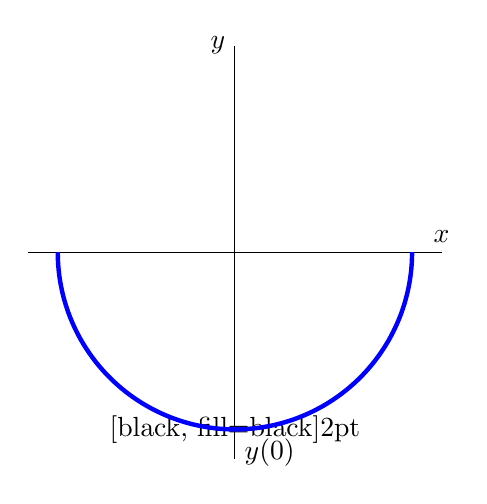
\begin{tikzpicture}[xscale=0.75,yscale=0.75]
	\draw[-{\seta}] (-3.5,0) -- (3.5,0) node[above] {$x$};
	\draw[-{\seta}] (0,-3.5) -- (0,3.5) node[left] {$y$};
	\draw[] (0,-3) node {\tikzcircle[black, fill=black]{2pt}};
	\draw[] (0,-3) node[below right] {$y(0)$};
  \draw[samples=100,ultra thick,domain=0:180,smooth,variable=\t,blue] plot ({3*cos(\t)},{-3*sin(\t)});
\end{tikzpicture}
	& 
	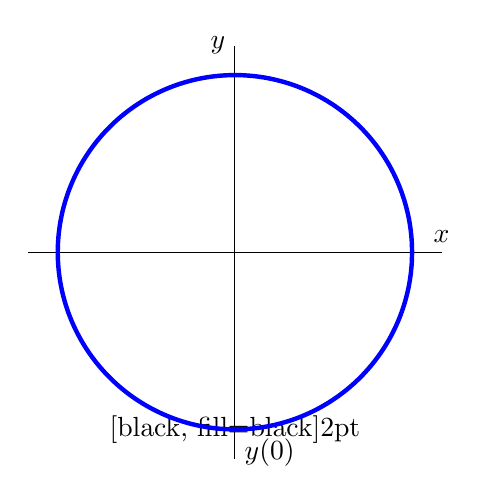
\begin{tikzpicture}[xscale=0.75,yscale=0.75]
		\draw[-{\seta}] (-3.5,0) -- (3.5,0) node[above] {$x$};
		\draw[-{\seta}] (0,-3.5) -- (0,3.5) node[left] {$y$};
		\draw[] (0,-3) node {\tikzcircle[black, fill=black]{2pt}};
		\draw[] (0,-3) node[below right] {$y(0)$};
	  \draw[samples=100,ultra thick,domain=0:360,smooth,variable=\t,blue] plot ({3*cos(\t)},{-3*sin(\t)});
	\end{tikzpicture}

	\\
Solution of the initial-value problem
	& Integral curve for the initial-value problem
\end{tabular}
\end{center}





\end{example}



	\begin{exercises}
		% Topics:
		% 
	\begin{problist}
	\prob Check that curves of the form $x^2 + y^2 = C$ satisfy the differential equation $\dfrac{dy}{dx} = -\dfrac{x}{y}$.
	
	
	\prob Is the piecewise-defined function
	$$
	y(x) = \begin{cases}
 		-x^2 & \text{ if } x< 0 \\
 		x^2 & \text{ if } x \geq 0		
	\end{cases}
	$$
	a solution of the differential equation $xy'-2y=0$ on $(-\infty,\infty)$?
	
	
	\prob Consider the differential equation
	$$ y^{(4)} - 8y^{3)} + 26 y'' - 40y'+25y=0.$$
	
	\begin{enumerate}
		\item Is $y=4 e^{2x}\sin(x)$ a solution?
		\item Is $y=-8 x e^{2x}\cos(x)$ a solution?
		\item For the two function above, if they are solutions, what are initial conditions of the form
			\begin{itemize}
				 \item[] $y(0) =$
				 \item[] $y'(0) =$
				 \item[] $y''(0) =$
				 \item[] $y'''(0) =$
			\end{itemize}
			that the solution satisfies?
	\end{enumerate}


	\prob Consider the functions
	\begin{align*}
		f(x) & = 3x + x^2 	& g(x) & = e^{-7x} \\
		h(x) & = \sin(x) 	& j(x) & = \sqrt{x} \\
		k(x) & = 8 e^{3x}	& \ell(x) & = -2 \cos(x)
	\end{align*}
	
	Match each differential to one or more functions which are solutions.
	
	\begin{enumerate}
		\item $y'=3y$
		\item $y''+9y'+14y=0$
		\item $y''+y=0$
		\item $2x^2y'' + 3xy'=y$
	\end{enumerate}
	
	
	
	\prob Consider the differential equation $u' = -2(u-10)$.
	
	\begin{enumerate}
		\item Check that the curves of the form $u = 10 + C e^{-2t}$ satisfy the differential equation.
		\item Sketch one solution of the differential equation.
		\item Sketch all the integral curves for the differential equation.
		\item What is the difference between a solution passing through the point $(1,20)$ and an integral curve passing through the same point?
	\end{enumerate}


	\prob Consider the differential equation $y'\big( 3y^2-1\big) = 1$.
	
	\begin{enumerate}
		\item Check that the curves of the form $y^3-y=x+C$ satisfy the differential equation.
		\item Sketch the solution of the differential equation that passes through $(1,1)$.
		\item Sketch the integral curve for the differential equation that passes through $(1,1)$.
		\item What is the difference between a solution passing through the point $(1,1)$ and an integral curve passing through the same point?
		\item Repeat (b)--(d) with the points $(1,0)$ and $(1,-1)$ instead of $(1,1)$.
	\end{enumerate}


	\prob Consider the ODE \quad $y'(t) = \big(y(t)\big)^2$ \quad .
	One of these two graphs {\bf cannot} describe the solution. 
	Which one? 
	
	
	\begin{center}
	\begin{tikzpicture}
		\draw[-{\seta}] (-1,0) -- (3,0) node[above] {$t$};
		\draw[-{\seta}] (0,-3) -- (0,1) node[left] {$y$};
		\draw[ultra thick,domain=0.5:2.5,smooth,variable=\x,blue] plot ({\x},{(\x*\x-5)/3-1});
	\end{tikzpicture}
	\hfil
	\begin{tikzpicture}
		\draw[-{\seta}] (-1,0) -- (3,0) node[above] {$t$};
		\draw[-{\seta}] (0,-3) -- (0,1) node[left] {$y$};
		\draw[ultra thick,domain=0.5:2.5,smooth,variable=\x,blue] plot ({\x},{-((\x-3.5)^2)/4-0.25});
	\end{tikzpicture}	
	\end{center}

	\prob We seek a first-order ordinary differential equation \quad $y' = f(\pmb{y})$ \quad whose solutions satisfy
	$$
	\begin{cases}
	y(x)  \mbox{ is concave up if } y < 1 \\
	y(x) \mbox{ is concave down if } y > 1
	\end{cases}
	$$
	%
	Write down or graph a function $f(y)$ that would produce such solutions.

	
	\end{problist}
\end{exercises}

\end{module}



\begin{lesson}
	\Title{Solutions}

	\Heading{Objectives}
	\begin{itemize}
		\item The second step in Mathematical modelling is to construct a representation of how the team will be attempting to solve the problem.
		\item Create a mind map of the problem. This is a structured way to brainstorm possible solutions and their requirements.
	\end{itemize}
	
	\Heading{Motivation} 

\begin{annotation}
	\begin{goals}
	\Goal{Extra Reading}
	Math Modelling: Getting started and getting solutions, Bliss-Fowler-Galluzzo
	
	\hfill \qrcode{https://m3challenge.siam.org/resources/modeling-handbook}	
	\end{goals}
\end{annotation}
	\Heading{Extra Reading} \href{https://m3challenge.siam.org/resources/modeling-handbook}{Math Modelling: Getting started and getting solutions, Bliss-Fowler-Galluzzo}

\end{lesson}




\newpage

\question

Which of these shows solutions of $y' = (x-1)(x+1) = x^2 - 1$ ?

\newlength{\len}
\setlength{\len}{120pt}
\begin{tabular}{ccc}
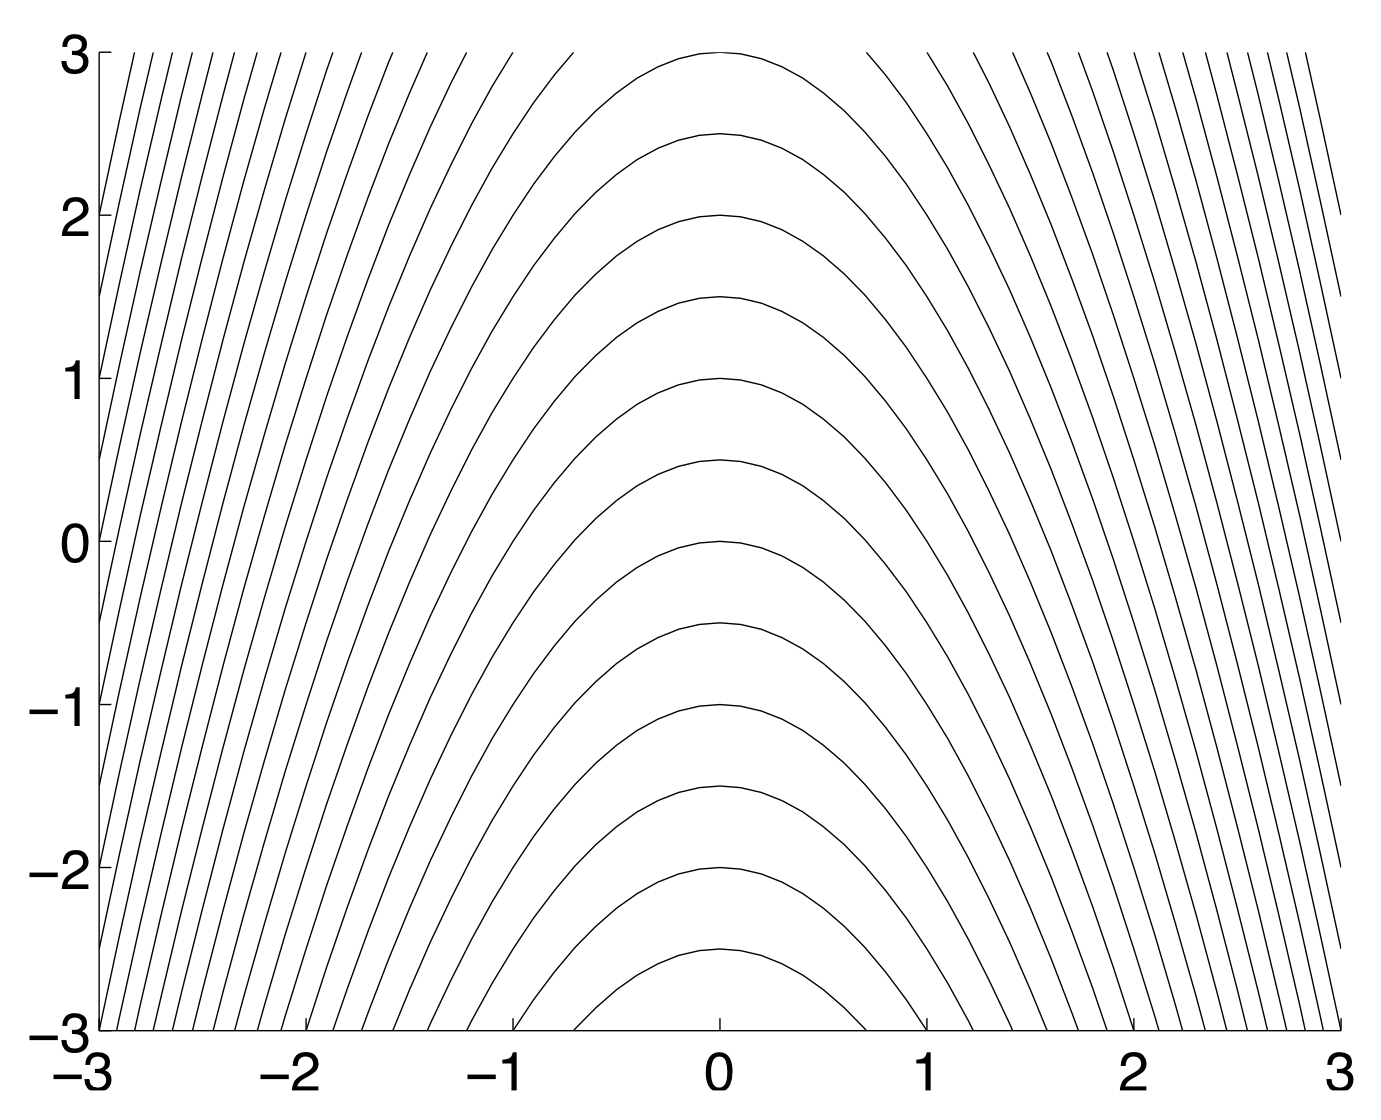
\includegraphics[width=\len]{images/module8-figs-6.png}
	& 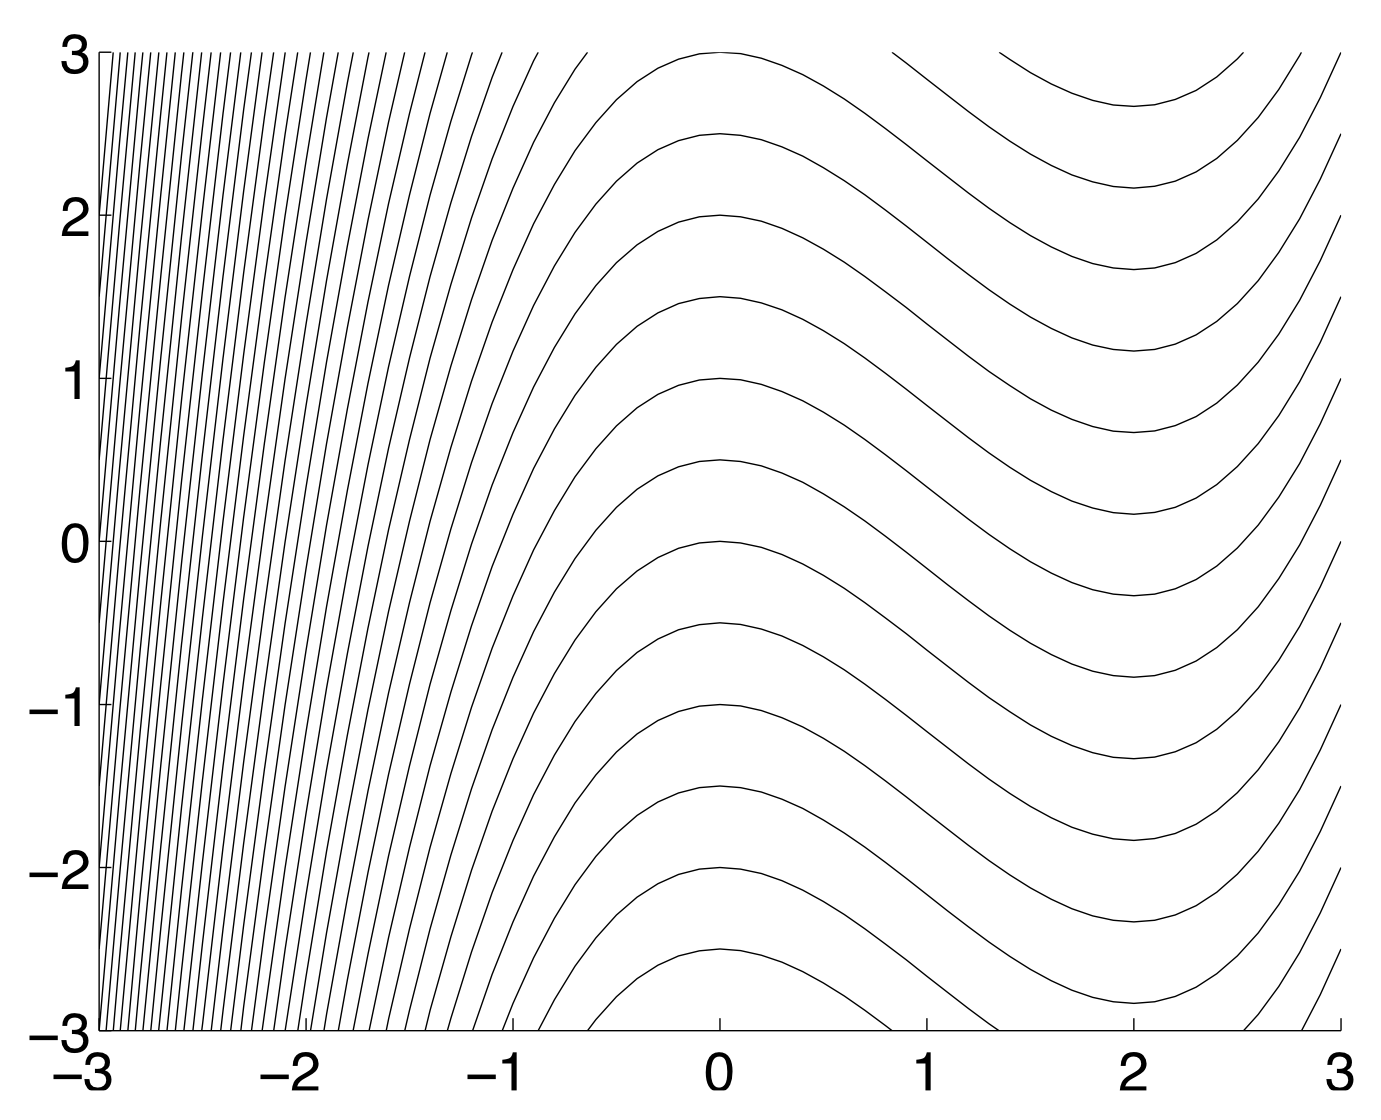
\includegraphics[width=\len]{images/module8-figs-3.png}
	& \includegraphics[width=\len, page=2]{images/module8-figs-2.png} \\
A & B & C \\[15pt]
%
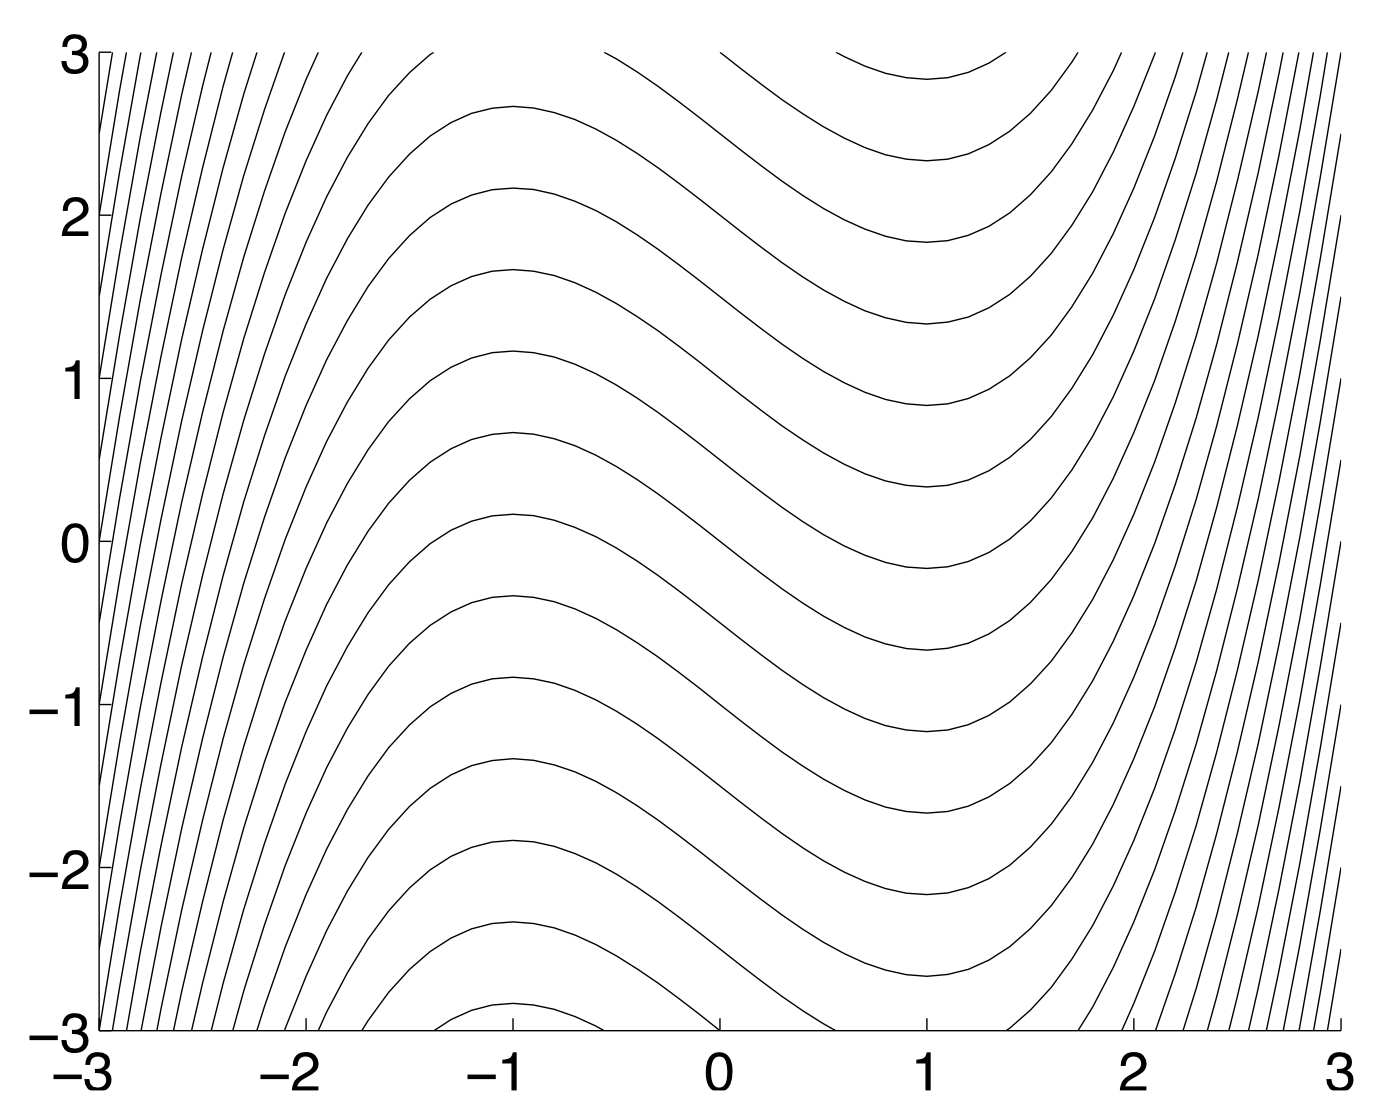
\includegraphics[width=\len]{images/module8-figs-1.png}
	& 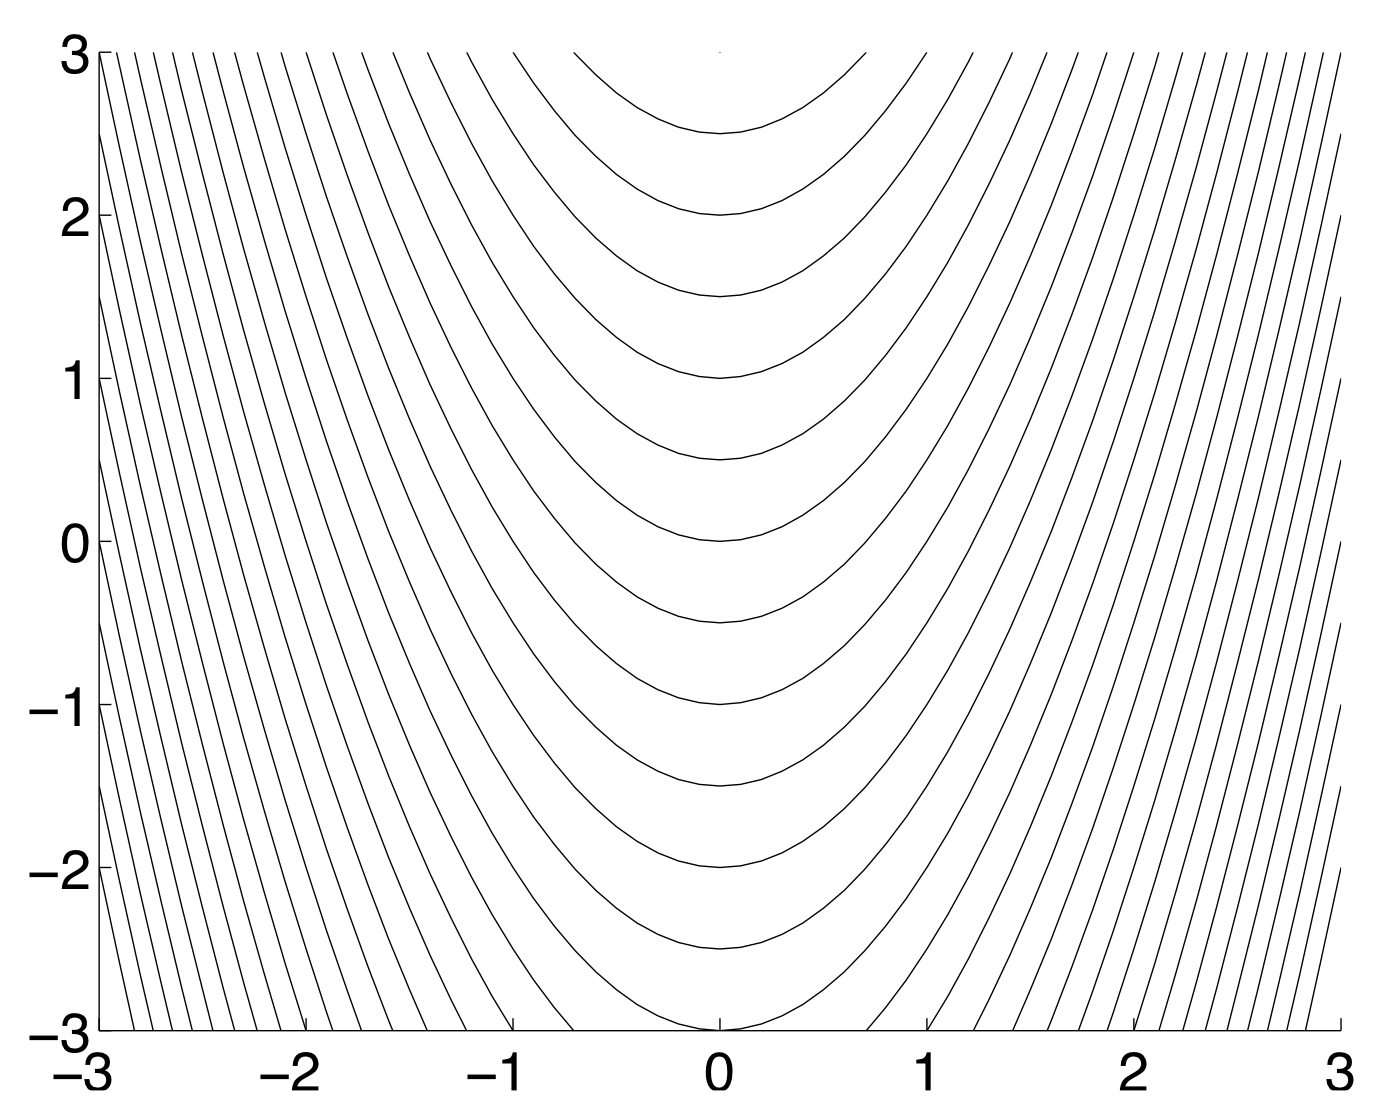
\includegraphics[width=\len]{images/module8-figs-5.png}
	& 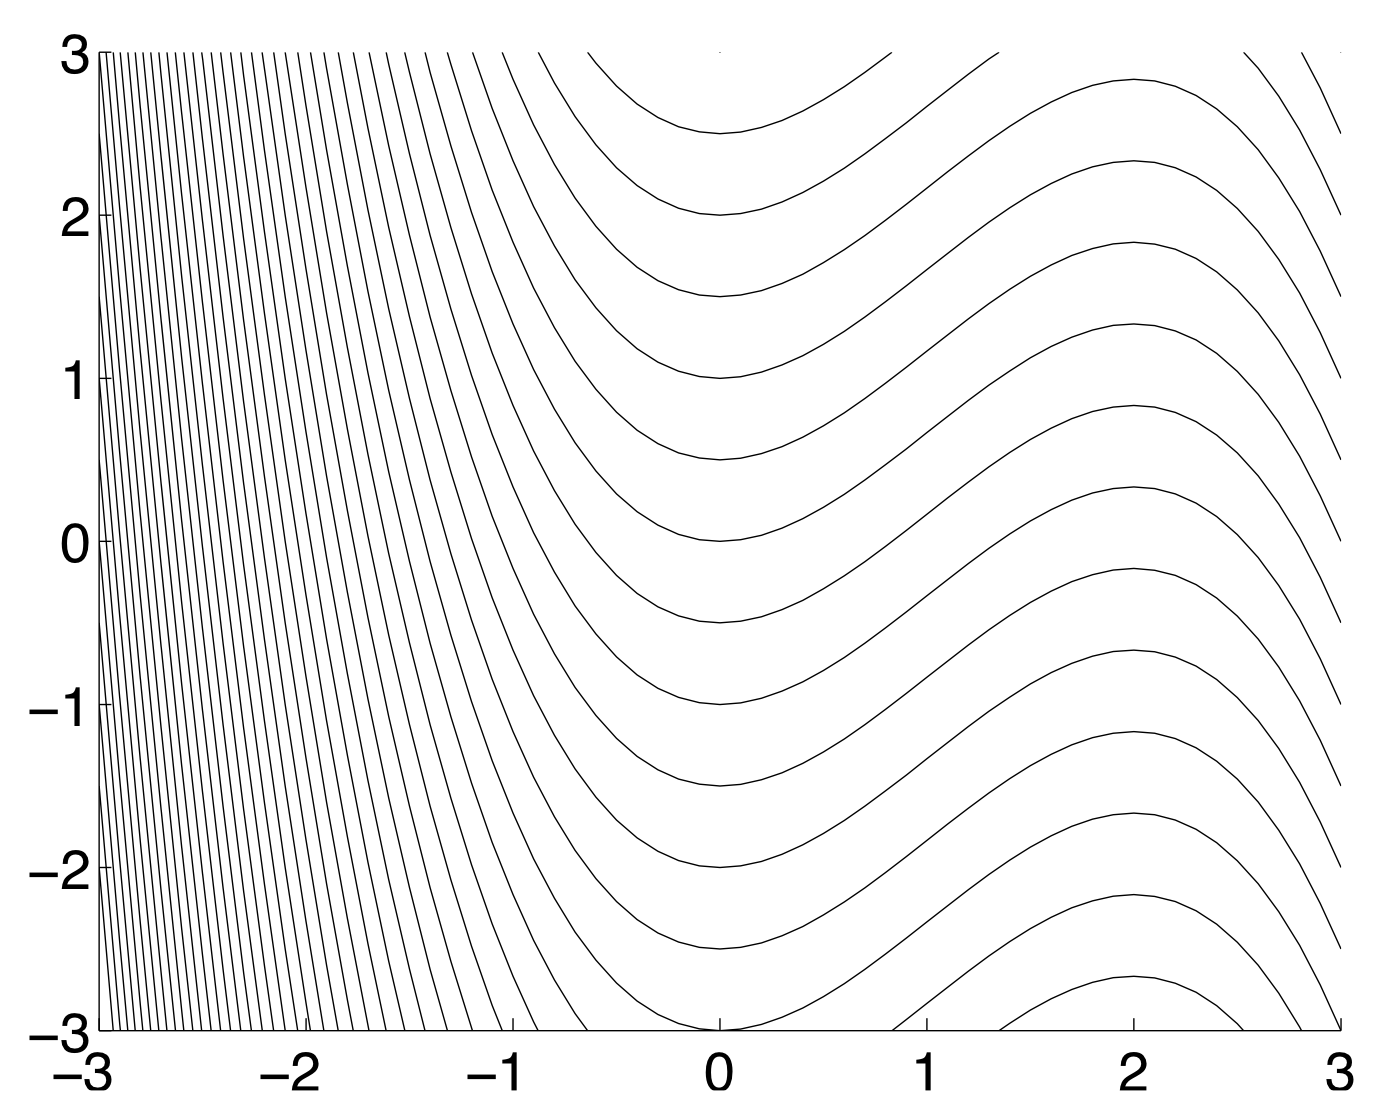
\includegraphics[width=\len]{images/module8-figs-4.png} \\
D & E & F \\
\end{tabular}

%		\begin{tabular}{ccc}
%		%	\begin{tikzpicture}
%		%	    \begin{scope}
%		%	    \clip (-3,-3) rectangle (3,3);
%		%		\foreach \k in {-9,-8, ..., 36} {
%		%	      \draw[samples=50,domain=-3:3,variable=\x] plot ({\x},{\k/3-(\x*\x)});
%		%	    }
%		%	    \end{scope}
%		%	    \draw[thick] (-3,-3) -- (-3,3);
%		%	    \draw[thick] (-3,-3) -- (3,-3);
%		%	    \foreach \k in {-3,-2, ..., 3} {
%		%	      \draw ({\k,-3}) node[below] {\tiny $\k$};
%		%	      \draw ({-3,\k}) node[left] {\tiny $\k$};
%		%	    }
%		%	\end{tikzpicture}
%		\includegraphics[width=\len, page=6]{images/module8-figs.pdf}
%			& \includegraphics[width=\len, page=3]{images/module8-figs.pdf}
%			& \includegraphics[width=\len, page=2]{images/module8-figs.pdf} \\
%		A & B & C \\[15pt]
%		%
%		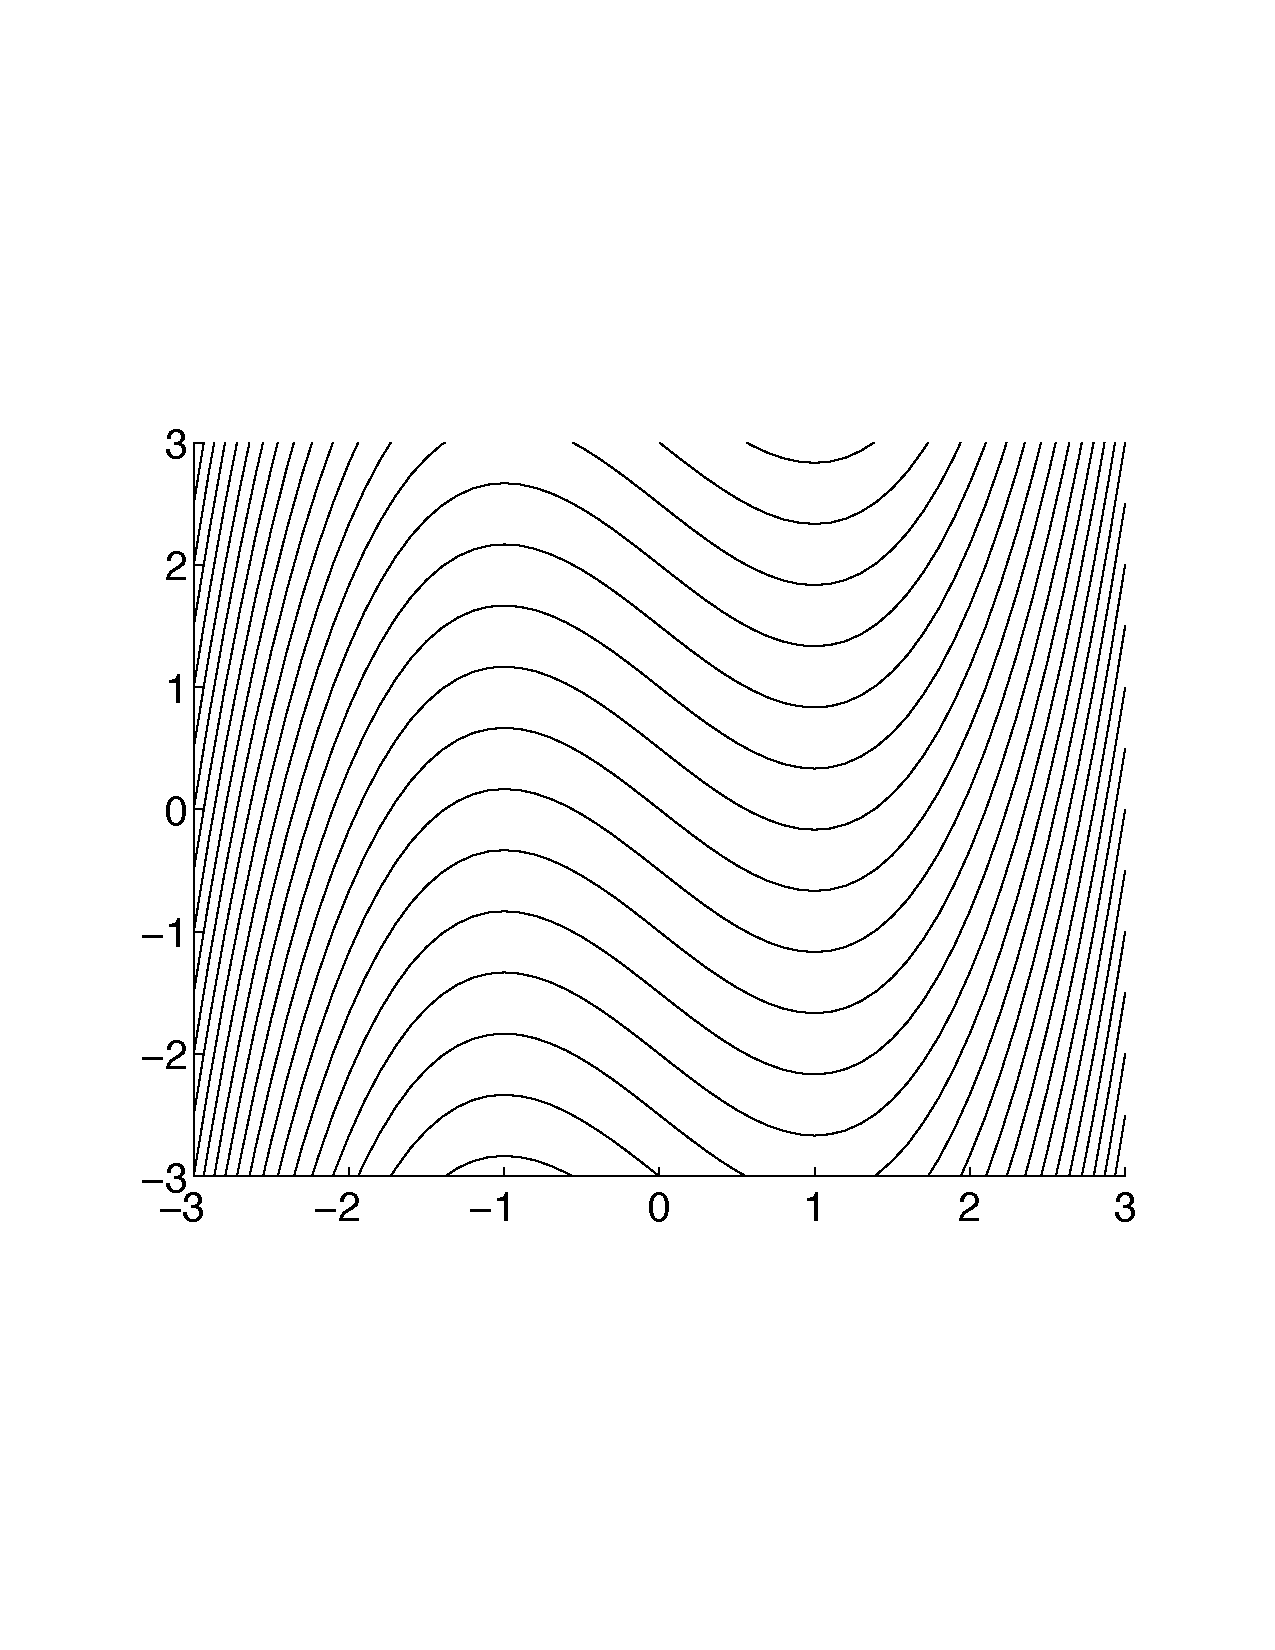
\includegraphics[width=\len, page=1]{images/module8-figs.pdf}
%			& 
%		%		\begin{tikzpicture}
%		%	    \begin{scope}
%		%	    \clip (-3,-3) rectangle (3,3);
%		%		\foreach \k in {-9,-8, ..., 36} {
%		%	      \draw[samples=50,domain=-3:3,variable=\x] plot ({\x},{-\k/3+(\x*\x)});
%		%	    }
%		%	    \end{scope}
%		%	    \draw[thick] (-3,-3) -- (-3,3);
%		%	    \draw[thick] (-3,-3) -- (3,-3);
%		%	    \foreach \k in {-3,-2, ..., 3} {
%		%	      \draw ({\k,-3}) node[below] {\tiny $\k$};
%		%	      \draw ({-3,\k}) node[left] {\tiny $\k$};
%		%	    }
%		%	\end{tikzpicture}
%		\includegraphics[width=\len, page=5]{images/module8-figs.pdf}
%			& \includegraphics[width=\len, page=4]{images/module8-figs.pdf} \\
%		D & E & F \\
%		\end{tabular}


\bookonlynewpage


\question

We seek a first-order ordinary differential equation 
\quad $y' = f(x)$ \quad 
whose solutions satisfy
$$
\begin{cases}
y(x)  \mbox{ is increasing if } x<2 \\
y(x) \mbox{ is decreasing if } 2 < x < 4 \\
y(x) \mbox{ is increasing if } x > 4
\end{cases}
$$
%
Write down or graph an $\pmb{f(x)}$ that would produce such solutions.




\bookonlynewpage

\question

Consider the ODE \quad $y'(t) = \big(y(t)\big)^2$ \quad .
Which of the following is true?
	
\begin{parts}
	\item $y(t)$ must always be positive
	\item $y(t)$ must always be negative \\[5pt]

	\item $y(t)$ must always be decreasing
	\item $y(t)$ must always be increasing
\end{parts}




\bookonlynewpage

\question Consider the differential equation $2xy'=y$.
	
	\begin{parts}
		\item Check that the curves of the form $y^2 + C x = 0$ satisfy the differential equation.
		\item Sketch one solution of the differential equation.
		\item Sketch all the integral curves for the differential equation.
		\item What is the difference between a solution passing through the point $(1,-1)$ and an integral curve passing through the same point?
	\end{parts}








%%%%%%%%%%%%%%%%%%%%%%%%%%%%%%%%%%%%%%%%%%%%%%%%%%%%%%%%%%%%%%%%%%%%%%%%
%		Slope Fields



%%%%%%%%%%%%%%%%%%%%%%%%%%%%%%
%
%  MODULE - Slope Fields
%
%%%%%%%%%%%%%%%%%%%%%%%%%%%%%%



\begin{module}{Slope Fields}
	%\Title{Slope Fields}
	\label{intro-slopefields}

	In this module you will learn
\begin{itemize}
	\item what is a slope field
	\item how to sketch a slope field
	\item to interpret a slope field
\end{itemize}

\hfill \\

As we saw in the previous module, once we have found a differential equation that models a situation, we often want to figure out what happens to the solution.

In this module, we will focus on getting an idea of the solutions and integral curves using what is called a \textbf{slope field}.





\begin{definition}[Slope field] Consider the equation $y' = f(x,y)$.
If we evaluate $f(x,y)$ over a rectangular grid of points, and we draw an arrow at each point $(x,y)$ of the grid with slope $f(x,y)$, then the collection of all the arrows is called a \emph{slope field}.
\end{definition}

\begin{graybox}
	
We can sketch Slope Fields with Wolfram Alpha.

For a differential equation $\dfrac{dy}{dx} = f(x,y)$, we need to input
\begin{itemize}
	\item Vector Field: $(1, f(x,y))$.
\end{itemize}

\url{http://www.wolframalpha.com/input/?i=slope+field}
\hfill \qrcode{http://www.wolframalpha.com/input/?i=slope+field}	
\end{graybox}





\begin{example}
Let us take an \hyperlink{sols-ex}{example from the previous module}.

Consider the initial-value problem
$$
\begin{cases}
	\dfrac{dy}{dx}=-\dfrac{x}{y} \\
	y(0)=-3
\end{cases}
$$

We can use this definition to sketch the slope field for the differential equation $ \dfrac{dy}{dx} = -\dfrac{x}{y}$.

We now sketch this slope field with Desmos:

\url{https://www.desmos.com/calculator/scmz6ps0or} \hfill \qrcode{https://www.desmos.com/calculator/scmz6ps0or}

Now notice that the arrows have the slope of a solution. This means that solutions will be tangent to the arrows, so we can \emph{roughly} trace the solution by following the arrows.

Below, we did just that starting with the point $(0,-3)$.

\setlength{\len}{175pt}
\begin{center}
%\begin{figure}
%\includegraphics*[width=\len]{images/module9-slopefield-ex1.png}
%\hfil
\begin{tabular}{ccc}
\includegraphics*[width=\len]{images/module9-slopefield-ex1-sol.png}
 & & 
\includegraphics*[width=\len]{images/module9-slopefield-ex1-intcurve.png}\\
approximated solution & & approximated integral curve
\end{tabular}
%\caption{Slope Field for the differential equation $\frac{dy}{dx} = -\frac{x}{y}$.
%\label{mod9-slopefield1}
%\end{figure}
\end{center}

\textbf{\textcolor{orange}{Important. }} Remember that this gives us only an approximation of the solution and integral curve. From the approximation, we can tell that the solution seems circular, but we still need to show that it is so.

\end{example}



%\setlength{\len}{150pt}
%\hspace{-1.35cm}\begin{tabular}{ccc}
%\includegraphics*[width=\len]{figures/0101_dirfield_rocket.png}
%	& \includegraphics*[width=\len]{figures/0101_intcurves_rocket.png} 
%	& \includegraphics*[width=\len]{figures/0101_rocket_pos.png} \\
%Direction field for $u$
%	& Approximations of $u$
%	& Solution $u(t)$
%\end{tabular}


%
%This particular one is:
%\href{http://www.wolframalpha.com/input/?i=direction+field+calculator&f1=%7B1%2C-9.8*x-0.75*y%2B10%7D%2Fsqrt(1%2B(-9.8*x-0.75*y%2B10)%5E2)&f=VectorPlot.vectorfunction%5Cu005f%7B1%2C-9.8*x-0.75*y%2B10%7D%2Fsqrt(1%2B(-9.8*x-0.75*y%2B10)%5E2)&f2=x&f=VectorPlot.vectorplotvariable1%5Cu005fx&f3=0&f=VectorPlot.vectorplotlowerrange1%5Cu005f0&f4=2&f=VectorPlot.vectorplotupperrange1_2&f5=y&f=VectorPlot.vectorplotvariable2%5Cu005fy&f6=0&f=VectorPlot.vectorplotlowerrange2%5Cu005f0&f7=4&f=VectorPlot.vectorplotupperrange2%5Cu005f4}{\tt Click Here}
%\hfill \qrcode{http://www.wolframalpha.com/input/?i=direction+field+calculator&f1=%7B1%2C-9.8*x-0.75*y%2B10%7D%2Fsqrt(1%2B(-9.8*x-0.75*y%2B10)%5E2)&f=VectorPlot.vectorfunction%5Cu005f%7B1%2C-9.8*x-0.75*y%2B10%7D%2Fsqrt(1%2B(-9.8*x-0.75*y%2B10)%5E2)&f2=x&f=VectorPlot.vectorplotvariable1%5Cu005fx&f3=0&f=VectorPlot.vectorplotlowerrange1%5Cu005f0&f4=2&f=VectorPlot.vectorplotupperrange1_2&f5=y&f=VectorPlot.vectorplotvariable2%5Cu005fy&f6=0&f=VectorPlot.vectorplotlowerrange2%5Cu005f0&f7=4&f=VectorPlot.vectorplotupperrange2%5Cu005f4}



\begin{video}
\begin{itemize}
	\item \href{https://youtu.be/MI2xCwBekX4}{https://youtu.be/MI2xCwBekX4} \hfill \qrcode{https://youtu.be/MI2xCwBekX4}
	\item \href{https://youtu.be/8Amgakx5aII}{https://youtu.be/8Amgakx5aII} \hfill \qrcode{https://youtu.be/8Amgakx5aII}
\end{itemize}	
\end{video}



	\begin{exercises}
		% Topics:
		% 
	\begin{problist}
	\prob Use Wolfram Alpha, Desmos, or another software to sketch the slope field for the following differential equations. Then roughly trace different solutions.
	\begin{enumerate}
		\item $y'=2y-x$
		\item $y'=xy$
		\item $y'=\cos(y)$
		\item $y'=\frac12+\cos(y)$
		\item $y'=1+\cos(y)$
		\item $y'=2+\cos(y)$
		\item $y'=\sin(xy)$
		\item $y'=\tan(x+y)$
	\end{enumerate}
	
	\prob Sketch a slope field for the following differential equation
	$$ y'=f(x,y)$$
	where 
	$$
	f(x,y) = \begin{cases}
 		-x & \text{ if } x< 1 \\
 		y & \text{ if } x \geq 1		
	\end{cases}
	$$

	\prob Sketch a slope field for the following differential equation
	$$ y'=f(x,y)$$
	where the function $f(x,y)$ satisfies all of the following properties:
	\begin{enumerate}
		\item $f(x,y)$ is continuous
		\item $f(x,y) > 0$ when $x>1$ and $y>1$
		\item $f(x,y) < 0$ when $x<-1$ and $y<-1$
		\item $f(x,y)$ depends only on $x$ when $x<-1$ and $y>1$
		\item $f(x,y)$ depends only on $y$ when $x>1$ and $y<-1$
	\end{enumerate}
	
	
	\prob 
		\begin{enumerate}
			\item On the slope field from the previous problem, show that there must exist a smooth continuous curve with horizontal lines.

			\item Show that the curve divides the $(x,y)$ plane in two parts.

		\end{enumerate}
	
	


	\prob Consider a differential equation 
	$$ y'=f(x,y)$$
	where the solutions satisfy
	$$ \lim_{x\to \infty} y(x) = 1.$$

	\begin{enumerate}
		\item What property must the slope field satisfy?

		\item Sketch a possible slope field for this differential equation.
	\end{enumerate}
	
	\end{problist}
\end{exercises}

\end{module}



\begin{lesson}
	\Title{Slope Fields}

	\Heading{Objectives}
	\begin{itemize}
		\item The second step in Mathematical modelling is to construct a representation of how the team will be attempting to solve the problem.
		\item Create a mind map of the problem. This is a structured way to brainstorm possible solutions and their requirements.
	\end{itemize}
	
	\Heading{Motivation} 

\begin{annotation}
	\begin{goals}
	\Goal{Extra Reading}
	Math Modelling: Getting started and getting solutions, Bliss-Fowler-Galluzzo
	
	\hfill \qrcode{https://m3challenge.siam.org/resources/modeling-handbook}	
	\end{goals}
\end{annotation}
	\Heading{Extra Reading} \href{https://m3challenge.siam.org/resources/modeling-handbook}{Math Modelling: Getting started and getting solutions, Bliss-Fowler-Galluzzo}

\end{lesson}




\newpage

\question
\begin{minipage}{.7\textwidth}
	A catapult throws a projectile into the air and we track the height (in metres) of the projectile from the ground as a function $y(t)$, where $t$ is the time (in seconds) that elapsed since the object was launched from the catapult. \\

	Then, the slope fields for $y(t)$ and $y'(t)$ are shown below:
\end{minipage}\hfill
\begin{minipage}{100pt}
	\includegraphics*[width=100pt]{images/module9-catapult.pdf}	
\end{minipage}






\setlength{\len}{200pt}
\begin{tabular}{cc}
\includegraphics*[height=\len]{images/module9-y.png}
	& \includegraphics*[height=\len]{images/module9-yprime.png} \\
Slope field for $y(t)$
	& Slope field for $y'(t)$
\end{tabular}

\hfill {\footnotesize(These slope fields were created using WolframAlpha)} \\

\begin{parts}
	\item On the slope field, sketch a \emph{possible} solution.	
	\item Consider the graph of $y(t)$. Does it form a parabola? Justify your answer.
\end{parts}

\begin{annotation}
	\begin{Goals}
		Students should think about the initial conditions.
		What is a possible value for $y(0)$? What is a possible value for $y'(0)$?
		Then sketch a possible solution that starts at those values. \\
		
		The equilibrium in the slope field for $y'(t)$ is called \emph{terminal velocity}. Some students might be able to identify it.
	\end{Goals}
\end{annotation}





\bookonlynewpage



\question Sketch the slope field for the following differential equations. 

\begin{parts}
	\item $y'=x$

\begin{annotation}
	\begin{Goals}
		The goal is not to be very accurate, but to capture the symmetry of each of these slope fields.
	\end{Goals}
	
\end{annotation}

	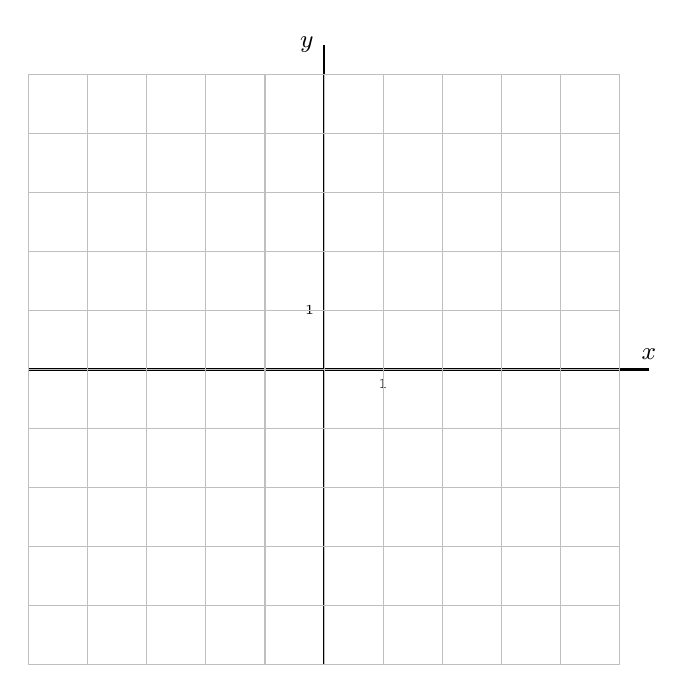
\begin{tikzpicture}[xscale=0.75,yscale=0.75]
		\draw[thick,-{\seta}] (-5,0) -- (5.5,0) node[above] {\small $x$};
		\draw[thick,-{\seta}] (0,-5) -- (0,5.5) node[left] {\small $y$};
		\draw[] (1,0) node[below] {\tiny 1};
		\draw[] (0,1) node[left] {\tiny 1};
		\draw[step=1,lightgray,thin] (-5,-5) grid (5,5);
	\end{tikzpicture}
	
	
\vfil	
	
	\item $y'=y^2$	

	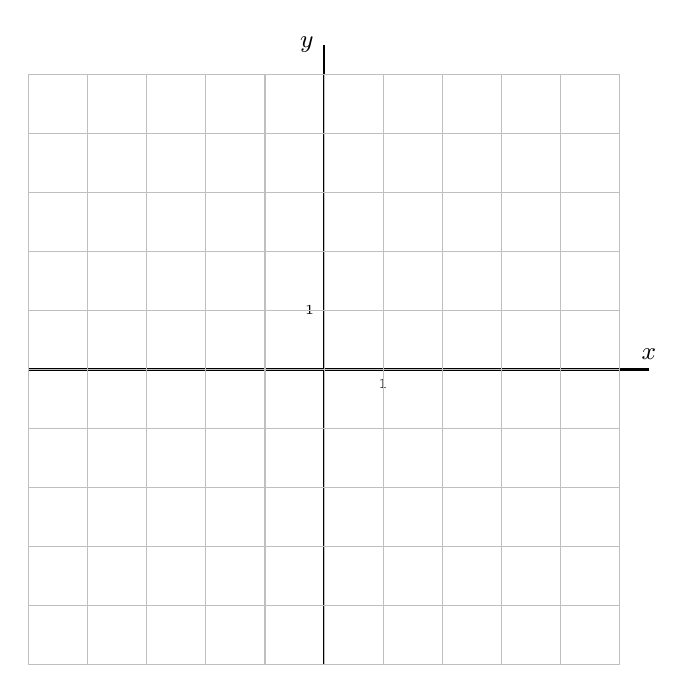
\begin{tikzpicture}[xscale=0.75,yscale=0.75]
		\draw[thick,-{\seta}] (-5,0) -- (5.5,0) node[above] {\small $x$};
		\draw[thick,-{\seta}] (0,-5) -- (0,5.5) node[left] {\small $y$};
		\draw[] (1,0) node[below] {\tiny 1};
		\draw[] (0,1) node[left] {\tiny 1};
		\draw[step=1,lightgray,thin] (-5,-5) grid (5,5);
	\end{tikzpicture}

\end{parts}



\bookonlynewpage

\question Consider the following slope fields:


\setlength{\len}{150pt}
\begin{tabular}{ccc}
	\includegraphics*[height=\len]{images/module9-graph1}
		& \includegraphics*[height=\len]{images/module9-graph2}
		& \includegraphics*[height=\len]{images/module9-graph3} \\
		(A) & (B) & (C) \\[10pt]
	\includegraphics*[height=\len]{images/module9-graph4}
		& \includegraphics*[height=\len]{images/module9-graph5}
		& \includegraphics*[height=\len]{images/module9-graph6} \\
		(D) & (E) & (F)
\end{tabular}

\hfill {\footnotesize(These slope fields were created using WolframAlpha)} \\


\begin{parts}
	\item Which slope field(s) corresponds to a differential equation of the form
		\qquad $y'=f(x)$ \qquad ?	

	\item Which slope field(s) corresponds to a differential equation of the form
		\qquad $y'=g(y)$ \qquad ?	

	\item Which slope field(s) corresponds to a differential equation of the form
		\qquad $y'=h(x+y)$ \qquad ?	

	\item Which slope field(s) corresponds to a differential equation of the form
		\qquad $y'=\kappa(x-y)$ \qquad ?	

	\item Which slope field(s) corresponds to a differential equation of the form
		\qquad $y'=1+\big( \ell(x,y) \big)^2$ \qquad ?	

	\item Which slope field(s) corresponds to a differential equation of the form
		\qquad $y'=1-\big( m(x,y) \big)^2$ \qquad ?	

\end{parts}

\begin{annotation}
	\begin{Goals}
		Students should be able to justify their choices	.
	\end{Goals}
	
\end{annotation}






\newpage




%%%%%%%%%%%%%%%%%%%%%%%%%%%%%%%%%%%%%%%%%%%%%%%%%%%%%%%%%%%%%%%%%%%%%%%%
%		Numerical Methods


\begin{module}{Numerical Methods}	
	%\Title{Numerical Methods}	
	\Heading{Objectives}
	\begin{itemize}
		\item Bla bla bla	
	\end{itemize}
	
	\Heading{Motivation} 


\end{module}





